\section{Einführung in Design Patterns}

Entwurfsmuster oder Design Patterns sind bewährte Lösungsansätze für wiederkehrende Probleme, die bei der Konzeption der Software-Architektur und während der Implementierung 
eingesetzt werden können. Dabei dienen diese Entwurfsmuster als eine Art Blaupause, die es Software-Entwicklern ermöglicht, erprobte Lösungsstrategien für häufig auftretende Probleme in der Software-Entwicklung anzuwenden.
Durch den Einsatz von etablierten Entwurfsmustern können Software-Entwickler für die Software bei korrekter Anwendung unter anderem erhöhte Wartbarkeit, Wiederverwendbarkeit von Komponenten, Verständlichkeit und Skalierbarkeit ermöglichen, was widerum in qualitativ besserer Software resultiert.
Dabei sollte beachtet werden, dass Design Patterns als Vorlage zu betrachten sind. Je nach Einsatzgebiet muss die Anwendung des Entwurfsmusters evaluiert und für den konkreten Fall individualisiert werden.
Deshalb existiert keine universelle anwendbare Iteration eines Design Patterns, die unabhängig von Anwendungskontext eingesetzt werden kann. Dies resultiert in variierender Anwendung von Entwurfsmustern, abhängig von jeweiligem Einsatzgebiet.
Im weiteren Entwicklungszyklus der Software werden durch neue oder geänderte Anforderungen bereits eingesetzte Implementierungen von Entwurfsmustern modifiziert, entfernt oder neue hinzugefügt.
Währenddessen besteht die Gefahr, dass durch mangelnde Dokumentation oder andere Gründe die Entscheidungen, weshalb Entwurfsmuster so eingesetzt sind, wie es eingesetzt worden sind, verloren gehen.
Dadurch besteht die Gefahr, dass angewendete Design Patterns im weiteren Verlauf der Entwicklung nicht mehr wiederzuerkennen sind. Deswegen ist die Etablierung eines Prozesses von Vorteil, der in der Lage ist,
Implementierungen von Entwurfsmustern aus einem Software-System zu extrahieren und diese konkret zu benennen. Vor allem der Einsatz von Machine Learning für die Klassifizierung ist hier vorteilhaft, wodurch das Potenzial besteht, vorher nicht gesehene Implementierung von Design Patterns zu erkennen.
Der Fokus dieser Arbeit besteht darin, solch einen Prozess zu etablieren, welcher für ein gegebenes Set von Quellcode-Dateien mithilfe von Machine Learning ein passendes Entwurfsmuster zuteilt. 

\pagebreak

\section{Untersuchungsfragen}

Das Ziel dieser Arbeit besteht aus der Etablierung eines Prozesses, womit durch Einsatz von Machine Learning für ein Set von Quellcode-Dateien ein Design Pattern zugeordnet wird.
Hierfür dienen eine Menge an Quellcode-Dateien als Eingabe für den Prozess und durch phasenweise Transformationen und Bearbeitungen sollen ein möglichst passendes Entwurfsmuster zugeordnet werden.
Um solch einen Prozess zu entwickeln, werden im Kontext dieser Arbeit folgende Fragen gestellt und beantwortet:

\begin{questions}
    \item\label{RQ1} Welche Design Patterns werden berücksichtigt?
    \item\label{RQ2} Was für ein Datensatz eignet sich für solch einen Prozess?
    \item\label{RQ3} Wonach wird exakt klassifiziert?
    \item\label{RQ4} Welche Merkmale, die aus Quellcode-Dateien extrahierbar sind, eignen sich für Klassifizierung durch Machine Learning Modelle?  
    \item\label{RQ5} Welche Klassifizierer eignen sich?
    \item\label{RQ6} Wie wird eine Instanz eines Entwurfsmusters bestimmt?
\end{questions}


\section{Übersicht der Methodik}

In diesem Abschnitt wird erläutert, wie die in dieser Arbeit vorgeschlagene Methodik aufgebaut ist. 
Diese ist dabei in zwei Teile aufzuteilen.

\begin{figure}[h]
    \centering
    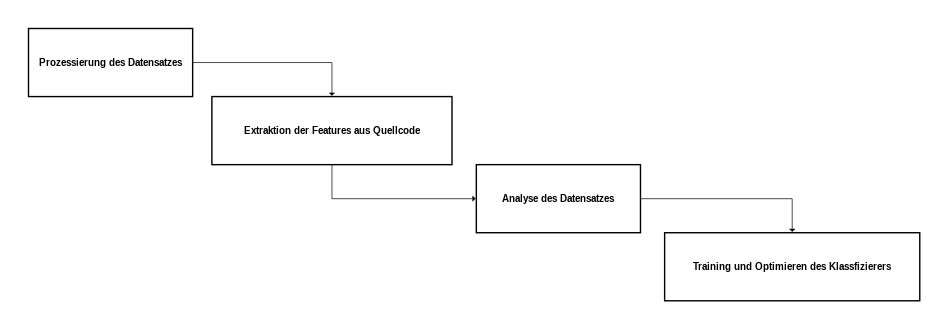
\includegraphics[scale=0.45]{figures/training_overview.png}
    \caption{Prozessabbildung des Trainings des Klassifizierers}
    \label{fig:training_process}
\end{figure}

Abbildung~\ref{fig:training_process} stellt die notwendigen Schritte dar, um einen Klassifizierer zu trainieren. Diese hat die Aufgabe,
Quellcodeentitäten eine Rolle im Kontext eines Entwurfsmusters zuzuordnen, das zu klassifizieren ist. Im ersten Schritt werden die notwendigen Informationen wie zugeordnetes Design Pattern und Rolle aus dem Datensatz extrahiert und in einer CSV-Datei abgelegt. 
Diese CSV-Datei dient zusammen mit dem eigentlichen Quellcode als Eingabe in der Feature-Extraktion in Form von Code-Metriken. Die Einträge aus der CSV-Datei werden dabei mit den berechneten Code-Metriken erweitert.
Darauffolgend wird eine explorative Datenanalyse durchgeführt, damit sich ein Überblick über die Datenpunkte geschafft wird. Anhand dieser Auswertung wird bestimmt, welche Entwurfsmuster und Rollen zur Klassifikation verfügbar sind.
Zum Schluss wird der verarbeitete Datensatz verwendet, um einen Klassifizierer zu trainieren. Der Trainingsschritt beinhaltet unter anderem die Optimierung des Modells durch Hyperparameter-Tuning und dessen Validation durch Kreuzvalidierung.
Die beste Iteration des Klassifizierers dient dabei als Grundlage bei der Bestimmung eines passenden Design Patterns.


\begin{figure}[h]
    \centering
    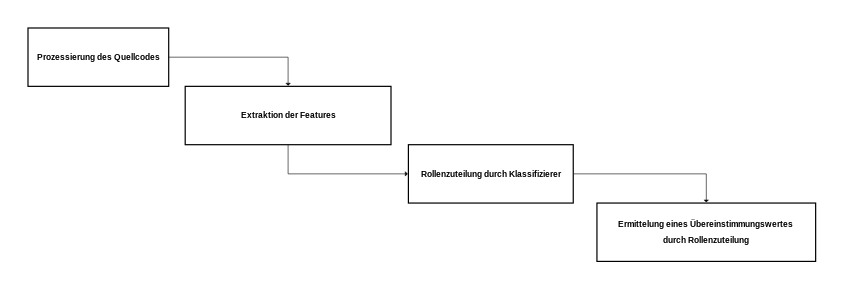
\includegraphics[scale=0.5]{figures/pattern_matching_overvierw.png}
    \caption{Prozessabbildung für Zuordnung von Entwurfsmustern}
    \label{fig:pattern_matching_overview}
\end{figure}

Die Abbildung~\ref{fig:pattern_matching_overview} beschreibt, wie auf Basis des vorher trainierten Klassifizierers ein Übereinstimmungswert ermittelt wird, der angibt,
welches Entwurfsmuster am ehesten zu den Quellcodeentitäten zuzuordnen ist. Wie im Trainingsprozess des Klassifizierers werden von den Quellcodeentitäten Code-Metriken extrahiert.
Diese werden als Eingabe für den Klassifizierer verwendet. Durch die Bestimmung der Rollen wird für jedes betrachtete Design Pattern ein Übereinstimmungswert berechnet.
Das Design Pattern mit dem höchsten Übereinstimmungswert ist das Entwurfsmuster, welches am ehesten zu dem Set an Quellcodeentitäten passt.

